\setchapterpreamble[u]{}
\chapter{Quality control}
\labch{QC}

\section{State of the Art in Spatial Transcriptomics Quality Control}

QC in ST is essential for identifying and removing technical artifacts such as tissue tears, low-quality spots, or poor sequencing depth, thereby ensuring reliable and reproducible gene expression data linked to precise spatial locations. It enables the distinction between true biological heterogeneity and technical noise, improving downstream analyses. QC procedures aim to remove low-quality spots or cells \sidenote{Spots in Visium and cells in Xenium} or technical artifacts before further analysis. Low-quality spots or cells can arise due to issues during library preparation or other experimental procedures. To avoid introducing unnecessary bias into downstream analyses, QC procedures are typically performed prior to subsequent steps. The main objective is the same as in any preprocessing pipeline in data analysis, with the added complexity that the biological nature of the data must be considered at every step.

As stated in \vrefch{intro}, this thesis focuses on the analysis of Xenium data. However, QC was first performed using Visium data as a simpler introductory step into QC for ST data. In the following two sections, the differences in the state of the art for both technologies are presented, with particular emphasis on the differences arising from how each technology acquires the data. Even slight changes in the way the biological complexity of a tissue is measured can substantially affect the QC procedures that follow.

\subsection{Quality Control in Visium-based approaches}
\labsec{QC_V}

This section outlines the QC and exploratory analysis workflow for 10x Genomics Visium ST data. Biological heterogeneity in single-cell and spatial RNA-seq data is often confounded by technical factors, including sequencing depth. The number of molecules detected in each cell can vary significantly, even within the same cell type. Therefore, the interpretation of RNA-seq data requires effective pre-processing and normalization to mitigate this technical variability.

A state-of-the-art review of QC methodologies for this type of data was conducted to establish a foundational understanding of transcriptomics QC. Most authors agree on the same core steps\sidenote{These steps are highlighted in black throughout this section}, differing mainly in the choice of R libraries\sidenote{This work was performed using \texttt{Seurat}, as the data structure was designed according to its requirements. Additionally, the expertise of the collaborating laboratory was with this library. Alternative libraries tested were more tailored to single-cell data and were insufficient for spatial applications.}, visualization strategies, and plotting approaches. Some workflows also include gene expression analysis as a final QC step\cite{MitocondrialExample}. However, since a dedicated section is provided for differential gene expression analysis (\vrefch{cellAnn}), this step is not included here.

The standard QC workflow for Visium data \cite{SeuratStandardWorflow} shares its main steps with Xenium and single-cell approaches, with slight modifications that will be discussed below.

The workflow begins by converting the raw sequencing reads (FASTQ files) into a spatially resolved gene expression count matrix using the Space Ranger pipeline, which constitutes the input data, which integrates high-throughput sequencing with histological imaging. In a bioinformatics context, this involves aligning a gene expression matrix (spots vs. genes) with a spatial coordinate system. From a biological perspective, this allows us to maintain the morphological context that is typically lost in dissociated single-cell RNA-seq (scRNA-seq). Every "spot" (approximately 55 $\mu$m in diameter) captures the transcriptomic profile of a small neighborhood of cells.

Once the data is loaded, \textbf{log-normalization} is required\cite{SeuratVisium}, as each spot captures a different total amount of RNA. This variability arises from technical variation, like:

\begin{itemize}
    \item Differences in sequencing depth: some spots get more reads\sidenote{Reads are NOT genes. They are short sequences of nucleotides that represent mRNA molecules within a tissue sample. A single gene can generate many overlapping reads.} simply because the group of cells in that spot had more transcripts in the moment of the experiment.
    \item Capture efficiency: some spots physically grab more RNA due to spot chemistry, cell denisty, artifacts, etc.
    \item Library preparation noise:\sidenote{In the context of RNA-seq, a library is a collection of DNA fragments, derived from the RNA sample, that have been prepared and optimized for sequencing on a specific platform} random distortions in the susequential steps after capturing the RNA.
\end{itemize}

Log-normalization rescales the counts to enable comparison of relative gene expression levels rather than total RNA abundance. This ensures that observed differences in gene expression are more likely to reflect biological variation rather than technical bias.

\begin{marginfigure}
	
\includegraphics{images/VisiumExample.png}
	\caption[Visium Example]{Example of a bladder cancer tissue analyzed with Visium 10x Genomics. Each dot represents a measurement spot containing multiple cells and transcripts. The color scale represents normalized expression levels (blue = low, yellow/red = high) of the gene NOC2L.}
\end{marginfigure}

The next step highlights a key difference between spatial and single-cell approaches: the \textit{removal of ribosomal and mitochondrial genes}. Due to the design of Visium and Xenium technologies\sidenote{Visium uses probe sets and Xenium uses targeted panels, meaning that the set of detectable genes is highly controlled}, these genes are typically not included unless specifically targeted. 

In contrast, in single-cell approaches, these genes are often removed because they constitute a large fraction of total RNA (ribosomal RNA accounts for approximately $\sim$80\textendash 90\% of total RNA, while mitochondrial genes can exceed 10\textendash 20\% of detected counts in stressed cells or spots), despite providing limited cell-type-specific information. Ribosomal genes reflect basic protein synthesis capacity, while mitochondrial genes are associated with energy metabolism and cellular stress or damage, not specialized cellular functions. Removing them during QC prevents these highly abundant housekeeping signals from dominating normalization and masking biologically meaningful spatial patterns. Nevertheless, some experiments incorporate these genes with the aim of using them as a filter in the QC \cite{MitocondrialExample}.

The next step involves \textbf{identifying highly variable genes}\sidenote{In this context, genes are referred to as features, as they constitute the variables used in downstream analyses.}. A highly variable gene is one whose expression level changes significantly across different cells, tissues, or experimental conditions, rather than remaining constant. The \verb|FindVariableFeatures| function from the \texttt{Seurat} R package identifies the most variable genes (typically the top 2000) across spots to capture biological heterogeneity. In other words, we are selecting genes that define cell-to-cell variation. This is achieved by modeling the mean-variance relationship and selecting genes that deviate from the expected trend\sidenote{Unlike usual data preprocessing, this step intentionally selects outliers. These genes form the basis of downstream analyses rather than being excluded.}. 

Despite normalization and feature selection, gene expression levels still vary widely. This variability reflects the underlying biological complexity and must be preserved. However, to prevent highly expressed genes from dominating downstream analyses and obscuring structural patterns, \textbf{data scaling} is required. Scaling centers gene expression (mean = 0) and standardizes variance (variance = 1) across spots, ensuring that all genes contribute equally to analyses such as principal component analysis (PCA) and clustering. Additionally, scaling allows the regression of unwanted technical variation.

The general idea is that normalization is performed first to correct for spot-level differences, followed by scaling to equalize gene contributions. This step is performed after feature selection because scaling transforms gene expression values, while \verb|FindVariableFeatures| is designed to operate on normalized or raw counts. Furthermore, this ordering improves computational efficiency\sidenote{Scaling in \texttt{Seurat} operates on each gene across all cells, making it dependent on sample structure rather than the total number of genes.}.

The final steps (normalization, variance stabilization, and feature selection) can also be performed simultaneously using the \verb|SCTransform| function\cite{SeuratVisium}, although it performs regularized negative binomial regression instead of conventional log-normalization. This function replaces \verb|NormalizeData|, \verb|ScaleData|, and \verb|FindVariableFeatures|. These steps represent the current state-of-the-art for QC in both single-cell and ST. While visualization methods and specific tools may vary, the essential components remain consistent: normalization, variance stabilization, and identification of highly variable features.


\subsection{Quality Control in Xenium-based approaches}
\labsec{QC_X}

As mentioned in \vrefsec{VisiumVSXenium}, Xenium is an image-based technology, since it enables the in situ detection of transcripts directly within the tissue thanks to multiplexed fluorescent microscopy. While Visium is a sequencing-based technology as it captures gene expression in spatial spots, Xenium provides subcellular resolution and assigns detected transcripts to individual cells after image segmentation. In most Xenium assays, the analysis is performed on a preselected panel of genes, although recent ST technologies are increasingly moving towards whole-transcriptome in situ profiling. This higher spatial resolution makes Xenium especially useful for studying tissue architecture and cell-to-cell organization, but it also introduces specific quality-control challenges related to image alignment, segmentation, transcript assignment and cell-level filtering. 

In general terms, the main steps of the QC workflow are similar to those used in Visium and scRNA-seq data: filtering low-quality cells, normalization, scaling, feature selection, dimensionality reduction, clustering and visualization. However, the way in which the results are validated differs depending on the technology. In Xenium, QC is not only based on transcriptomic metrics, but also on spatial and image-derived information, such as nuclei detection, cell segmentation quality and transcript localization.

Since Xenium is a more recent technology than Visium, there are fewer established libraries, benchmarks and standardized QC protocols available. Although several tutorials for downstream analyses are available online, the platform used to generate the data in this project recommends the use of \texttt{Seurat} for both Visium and Xenium data, with a particularly strong emphasis on Xenium workflows \cite{R4Xenium}. Downstream analyses can be performed both in R and Python, using libraries specifically adapted to ST. Nevertheless, R currently offers a wider and more mature ecosystem for transcriptomic data analysis, especially through packages such as \texttt{Seurat}, \texttt{SingleCellExperiment} and related Bioconductor tools.

As discussed in \vrefch{intro}, the novelty of Xenium makes the available options for data processing more limited than in the case of Visium. The main libraries used to analyze Xenium data are the aforementioned \texttt{Seurat} and \texttt{SingleCellExperiment}. The reasons for choosing \texttt{Seurat} are similar to those explained in \vrefsec{QC_V}. Nevertheless, both frameworks were explored during the development of this project.

A state-of-the-art review of QC methodologies for this type of data was conducted in order to establish a foundational understanding of transcriptomics QC. Most authors agree on the same core steps, although they differ in the choice of R libraries, visualization strategies and plotting approaches. Some workflows also include gene expression analysis as a final QC step. However, since this thesis includes a dedicated section for differential gene expression and cell annotation analysis in \vrefch{cellAnn}, this part is not included in the present QC section.

The standard computational workflow is similar to the one described in \vrefsec{QC_V}. It usually consists of normalization, scaling, feature selection, PCA, clustering, UMAP visualization and, when necessary, projection of the full dataset onto a reduced representation to accelerate the analysis. These steps can be performed with the same functions previously described for Visium and single-cell data. In some workflows, \texttt{SCTransform} is used instead of applying normalization, scaling and variance stabilization as separate steps. Conceptually, normalization corrects for differences in sequencing or detection depth between cells, while scaling makes gene expression values comparable across the dataset before dimensionality reduction and clustering.

However, Xenium data from the DUTRENEO clinical trial are considerably more memory-intensive than Visium data. This is due to the much larger number of cells, with approximately 5,399,355 cells and a panel size of 377 detectable genes per cell in Xenium, compared with around 99,028 Visium spots and 4,097 average unique genes per spot. Therefore, although each Xenium cell may contain fewer detected genes than a Visium spot, the total number of cellular observations makes the dataset much heavier computationally. For this reason, the analysis of large Xenium datasets, and also very large Visium datasets, may require the use of \verb|sketching|. Sketching, or intelligent subsampling, addresses scalability by selecting a small but representative subset of cells from the full dataset \cite{Ian.K.Gingerich}. The objective is to preserve both abundant and rare cell populations, maximizing variability, while reducing memory usage and computational time\sidenote{After sketching, the distribution of the data changes. This is the reason why scaling or recalibration steps must be repeated before continuing with downstream analyses.}. After sketching, the full dataset must be projected onto the dimensional reduction learned from the sketch. In \texttt{Seurat}, the function \verb|ProjectData| allows high-dimensional single-cell expression data from the full dataset to be projected onto the lower-dimensional embedding obtained from the sketched dataset.

At the cell level, two of the most common QC metrics are the total number of counts and the number of detected features. \sidenote{Note that, in this context, \textbf{counts} refer to the number of RNA molecules captured and sequenced in a given cell, whereas \textbf{features} refer to the genes that were captured and sequenced in that cell.} These metrics are used to identify low-quality cells, empty or poorly segmented regions, and possible technical artifacts. In Xenium, the total number of counts per cell is usually lower than in sequencing-based single-cell RNA-seq, because Xenium assays often target a predefined gene panel rather than the whole transcriptome. Therefore, filtering thresholds must be chosen according to the empirical distribution of each sample. A fixed upper threshold, such as 2,000 counts per cell, can be used as an initial reference, but it should not be interpreted as a universal rule. Instead, violin plots, histograms and spatial visualizations should be inspected to determine whether high-count outliers correspond to real tissue morphology or technical artifacts. For example, a sharp peak at unusually high count values may indicate problematic cells or regions that should be removed.

Another important group of QC metrics is based on control probes and control genes, which are molecules included in the Xenium assay to evaluate data quality and measurement accuracy. These controls provide reference signals with known expected behaviour, allowing the identification of technical artefacts and unreliable detections. Control genes correspond to endogenous transcripts whose expression can be used to assess sample quality, when they are designed to match something they are called positive control genes. For example, mitochondrial and ribosomal genes\sidenote{Already explained in \vrefsec{QC_V}}, can be used as indicators of cell quality. In addition to these positive biological controls, Xenium workflows may also include negative controls. Negative control probes are molecules designed to match nothing in the biological sample. If a negative probe 'lights up,' it is a mistake (likely caused by random background glow or the probe sticking to something it shouldn’t). By counting these false alarms, the system measures background noise and non-specific binding to identify false-positive detections in the experiment.  According to the Xenium literature cited in \cite{Voyager}, there are three main types of negative controls can be considered: probe controls, decoding controls and genomic DNA controls. 
\begin{itemize}
    \item Probe controls are used to assess non-specific binding to RNA.
    \item Decoding controls help estimate gene misassignment
    \item Genomic DNA controls are used to verify that the detected signal originates from RNA rather than DNA. 
\end{itemize}
Together, these controls provide an estimate of the false-positive rate in the experiment.

Other workflows, such as \cite{OSTA}, compute QC metrics based on the number of detected genes and the mitochondrial percentage with the aim of filtering low quality cells. The function \verb|addPerCellQCMetrics| from the \texttt{scuttle} package can conveniently add per-cell transcript counts, the proportion of total counts, and the number of detected features for selected gene subsets to a \texttt{SingleCellExperiment} object. Although this library has been updated to support ST data, currently it does not provide the same range of integrated spatial visualizations as more specialized packages. For this reason, the choice of library depends on the objective of the analysis: \texttt{SingleCellExperiment} is particularly useful for rigorous QC metric computation, whereas \texttt{Seurat} provides a more complete and integrated environment for visualization, clustering and downstream ST analysis.

Some workflows, such as those described in \cite{Voyager}, also use cell composition and segmentation-derived metrics as part of the QC process. The absence of nuclei can indicate technical artifacts or extreme stages of the cell life cycle; the cell might be dividing or dying at that moment. This represents a level of biological meaning that some approaches choose to extract, resulting in a further reduction of the data. For this reason, nucleus-based filtering should be interpreted carefully and, when possible, combined with spatial inspection of the tissue. Segmentation quality is especially relevant in Xenium. Since transcripts are assigned to cells according to segmentation boundaries, poor segmentation may lead to incorrect transcript assignment and, consequently, to misleading downstream analyses. A wrong segmentation can affect the apparent expression profile of a cell, alter clustering results and interfere with cell-type annotation. Nevertheless, severe segmentation problems are usually not restricted to a single isolated cell. If the segmentation or alignment is globally poor, it would be visible across the whole sample, as shown in \reffig{Good&Bad}. Therefore, segmentation quality should be assessed both quantitatively and visually.

\begin{figure}[H]
    \centering
    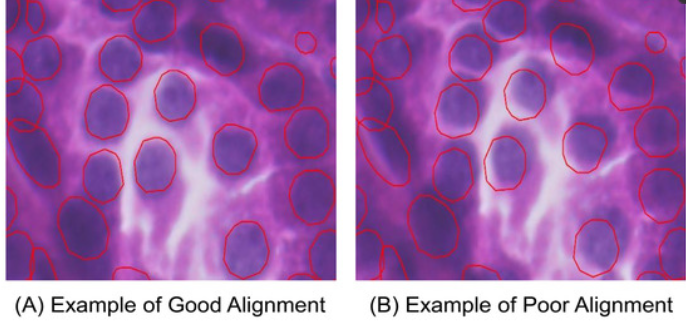
\includegraphics[width=\textwidth]{images/Godd&BadAllignment.png}
    \caption{Visualization of image alignment results in good and poor cases. \textbf{A} shows an example of good image alignment. \textbf{B} shows an example of poor image alignment. Image from \cite{Yu.Lin}.}
    \labfig{Good&Bad}
\end{figure}

\begin{figure}[H]
    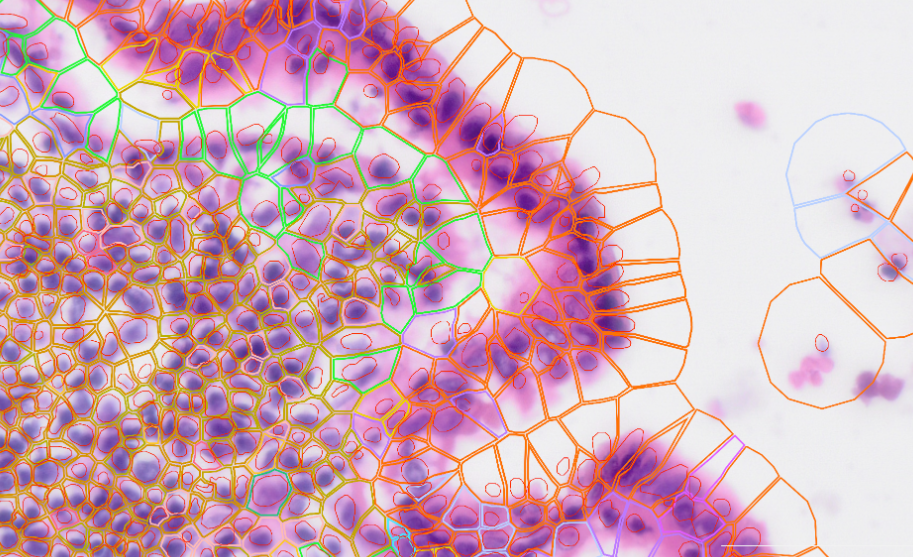
\includegraphics[width=\textwidth]{images/BadAllignment.png}
    \caption{Another example of poor alignment in Xenium. The cell and nuclei outlines show the result of a 15~\textmu m expansion distance for cell segmentation in the lumen of the human colon. Extracted from\\
    \url{https://www.10xgenomics.com/support/software/xenium-ranger/2.0/analysis/XR-import-segmentation}.
    The same tissue can be seen with label coloring in \vrefsec{Final_CellAnn} to better appreciate the structural organisation revealed by the annotations.}
 \end{figure}

Overall, the QC process in Xenium combines standard transcriptomic quality-control metrics with spatial and image-based validation. Counts, detected features and control probes provide information about the molecular quality of the data, while segmentation, nuclei detection and image alignment assess whether transcripts have been correctly assigned to cells within the tissue. This combination of molecular and spatial QC is essential to ensure that downstream analyses, such as clustering, cell annotation and differential gene expression, are biologically meaningful and not driven by technical artifacts.

\section{Final Methodology: Xenium-based Quality Control Pipeline}

As discussed in the previous section, \vrefsec{QC_X}, the choice of library depends on the objective of the analysis. For the final Xenium QC workflow, \texttt{Seurat} was selected because it allowed the integration of spatial visualization, cell-level metadata inspection, filtering, normalization, and downstream dimensionality reduction within the same analytical framework. Several complementary plots were used to identify potential outliers and technical artifacts while preserving biologically meaningful variation across samples.

\begin{marginfigure}%[-5.5cm]
    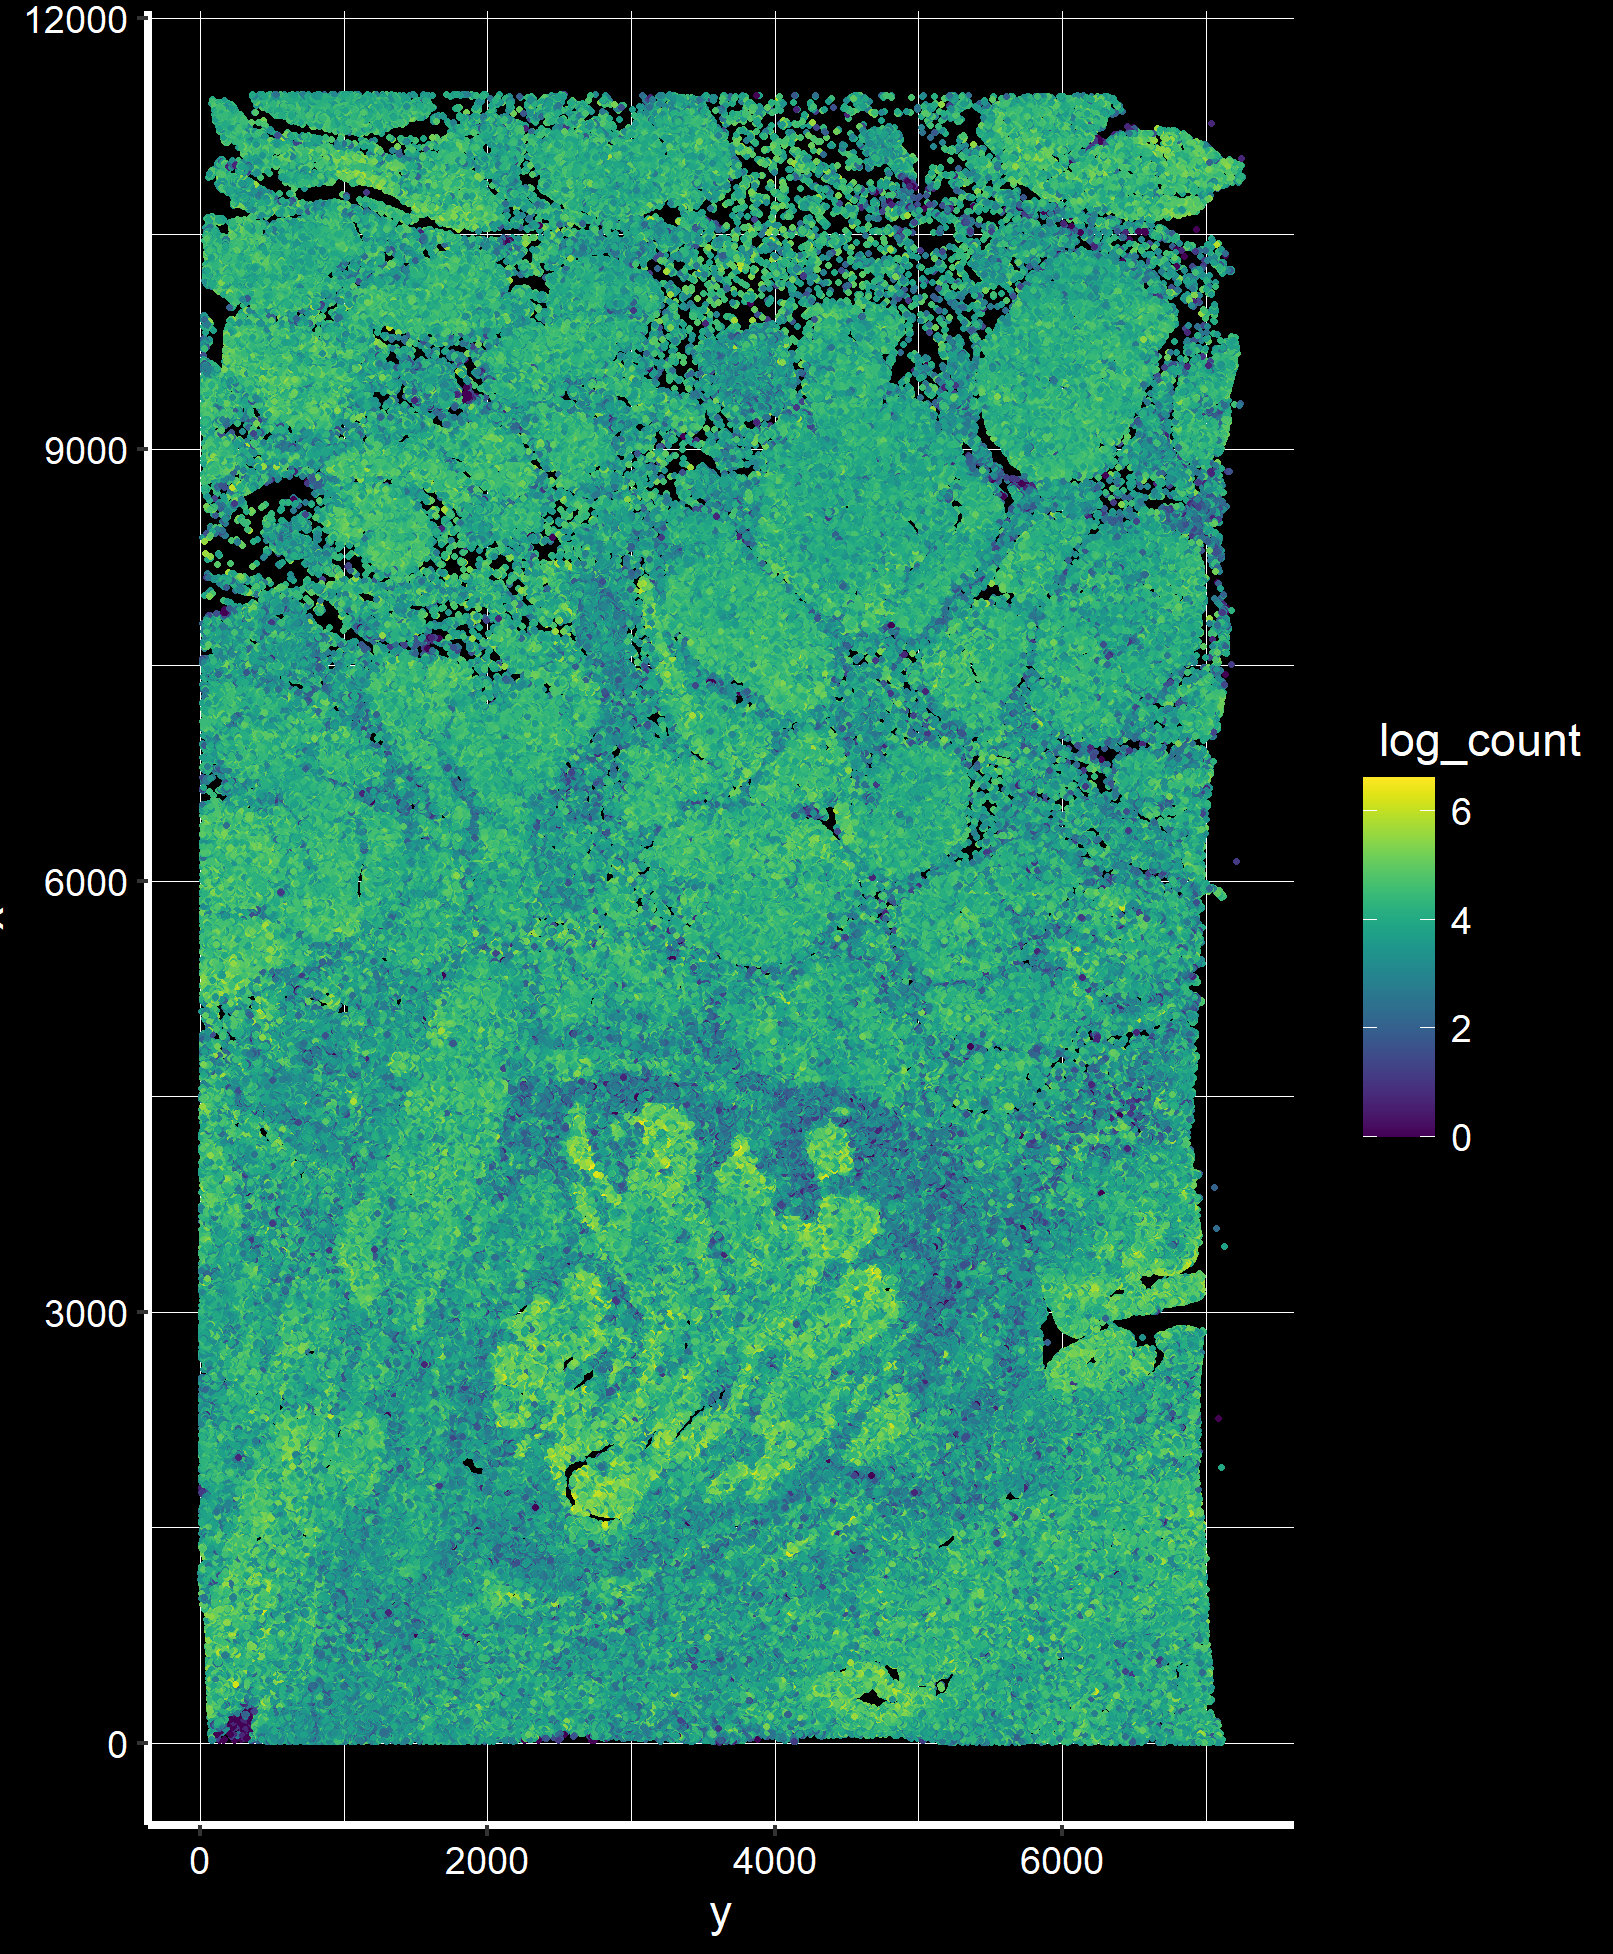
\includegraphics{images/Count_Intensity_x_region.png}
    \caption{Spatial distribution of \(\ln(1 + x)\)-transformed counts in sample DU53. The logarithmic transformation improves visualization by reducing the effect of extreme values while preserving numerical resolution across regions.} 
    \labfig{CountIntensityRegion}
\end{marginfigure}

A first and essential step was the spatial inspection of the cells within the tissue. Although this may seem basic, visualizing the spatial distribution of cells and transcript counts is crucial in Xenium data, where technical artifacts are often spatially structured. In particular, plotting the number of counts and features across tissue regions can reveal areas affected by folds, poor imaging, or local acquisition problems. Tissue folds may appear as irregular regions with abnormaly higher cell density and reduced transcript detection, because the folded area can not properly scanned and transcripts cannot be accurately assigned or decoded as the light can not get through the tissue.  

The next step in the final QC process made was looking for a count threshold. By plotting the distributions of the counts in each sample as shown in \reffig{CountDist}. The aim of this figure is to identify outlier or artifacts and select a natural threshold for our data.


After this spatial inspection, count distributions were evaluated across all samples in order to identify potential outliers and define a general upper-count threshold. The aim of this step was not only to remove extreme technical artifacts, but also to ensure that the retained cells represented realistic transcriptional profiles. As shown in \reffig{CountDist}, none of the samples displayed a clear extreme outlier distribution, and a threshold of 500 counts was selected as a sensitive and consistent cutoff across the dataset.

\begin{figure}[H]
    \centering
    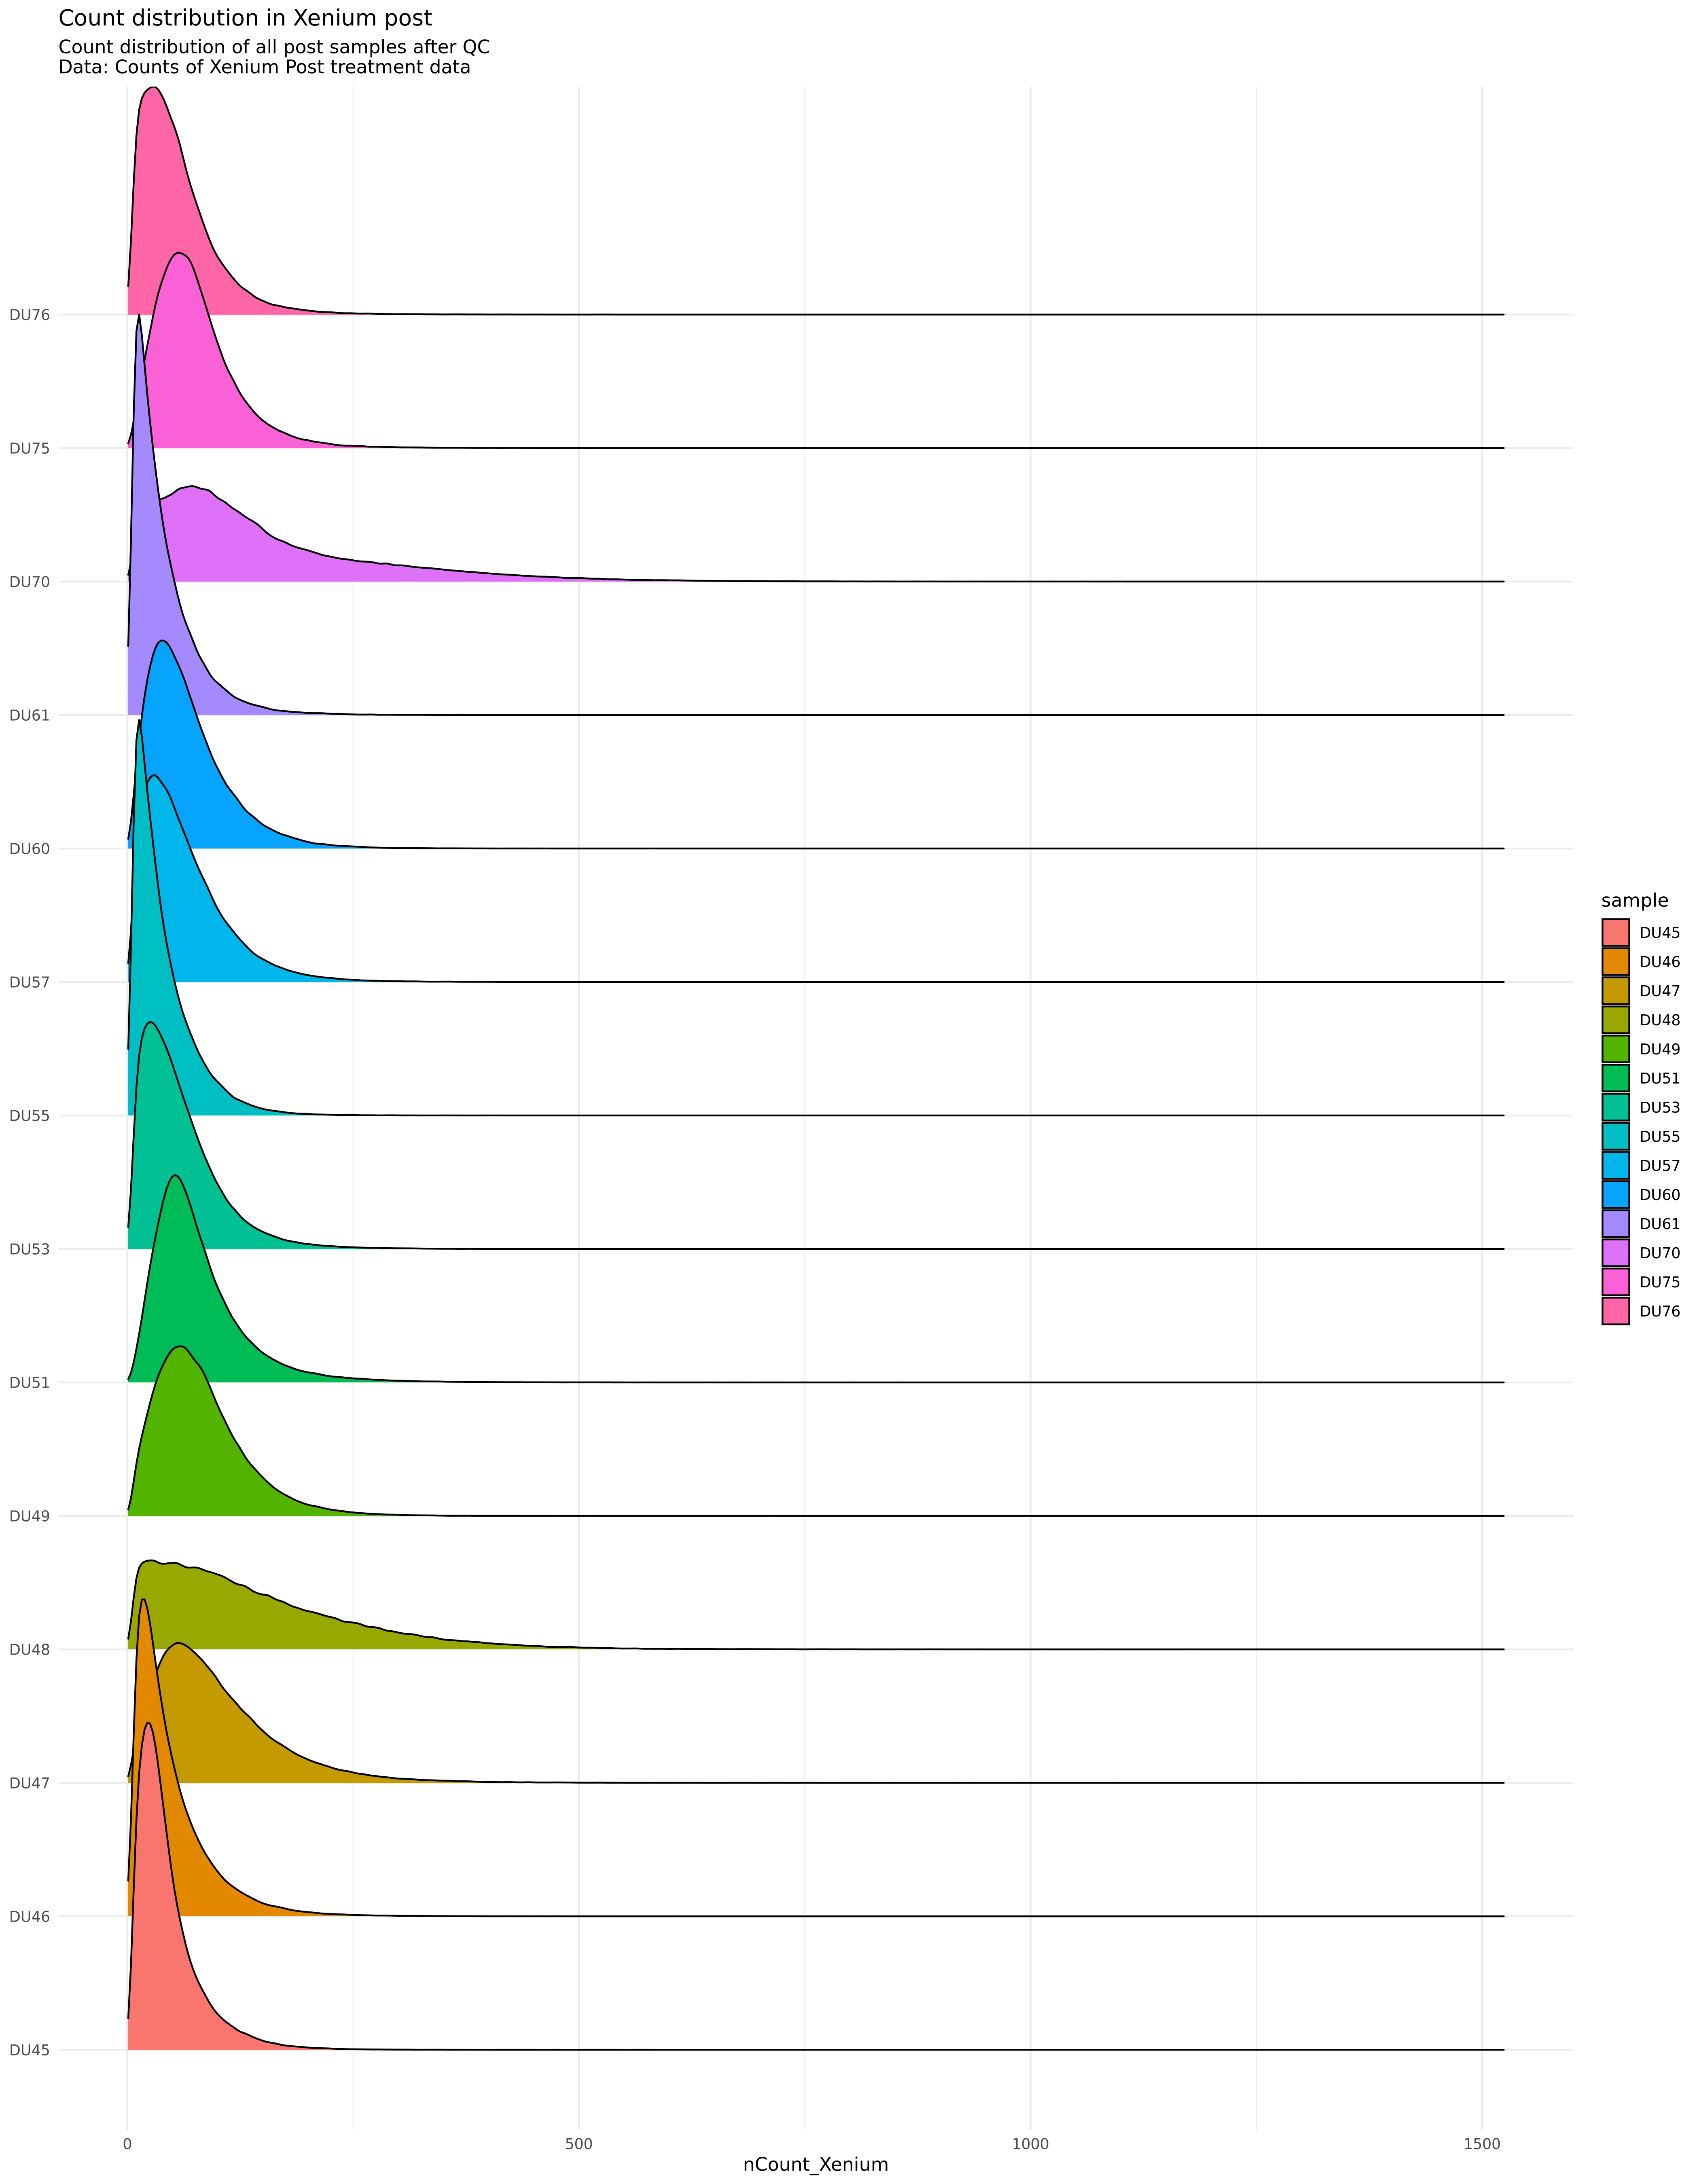
\includegraphics[width=\textwidth]{images/Count_distribution_ALLSAMPLES.png}
    \caption{Count distribution of all raw available samples, with each sample represented by a different color. No sample showed a strong outlier distribution, and 500 counts was selected as a sensitive upper threshold across samples.}
    \labfig{CountDist}
\end{figure}

The lower-count threshold was then assessed. Cells with very few detected transcripts are more likely to represent poor-quality segmentation, low-confidence transcript assignment, or incomplete cellular profiles. However, this threshold must be chosen carefully, since overly strict filtering can remove biologically relevant populations. For example, neutrophils are a cell type that naturally presents lower transcript counts, and a high lower-count cutoff could lead to the loss of an entire biologically meaningful population. For this reason, the lower threshold was set to \texttt{nCount\_Xenium > 5}, which removes cells with extremely low signal while minimizing the risk of excluding low-RNA but relevant cell types. This decision is also consistent with previously reported recommendations for Xenium QC \cite{Marco.Salas}.

Negative control probes were also considered as an additional quality metric. These probes, also referred to as negative controls\sidenote{Negative control probes are molecules designed not to match biological targets in the sample. If a negative probe is detected, this signal is likely caused by random background fluorescence, the probe binding to something it should not, or decoding error. The main types of negative controls include probe controls, decoding controls, and genomic DNA controls.}, are designed not to match any biological target in the sample. Therefore, signal detected from these probes reflects background noise, non-specific binding, or decoding errors rather than true biological expression. A high percentage of negative probe counts in a cell would therefore indicate unreliable transcript detection. A value above 10\% negative probes was considered a clear indication of poor-quality signal and would require filtering. However, in the present dataset, the maximum percentage observed was approximately 3\%, which was considered acceptable according to the tests reported in \cite{Marco.Salas}. Therefore, no additional filtering based on negative probe percentage was required.

Segmentation quality was also evaluated through the detection of isolated cells. In Xenium, nuclei are stained and an algorithm expands cell boundaries from the nuclear signal. When a nucleus is located far from other cells, especially in empty tissue regions or near the edge of the field of view, the resulting segmented cell area can become unrealistically large. These isolated segmented objects are often not representative of true cellular neighborhoods and may introduce noise into spatial analyses. Importantly, removing these cells is unlikely to eliminate transcripts from neighboring cells, since by definition they are spatially isolated and their assigned transcripts are expected to originate only from that isolated object. To identify these cases, different distance thresholds were evaluated, and cells with no neighbors within 70 \(\mu\)m were selected as isolated cells located outside or at the borders of the tissue.

\begin{figure}[H]
    \centering
    
\includegraphics[width=\textwidth]{images/Isolated_cells.png}
    \caption{Visualization of cells with no neighboring cell within 70 \(\mu\)m, shown as black dots. Plotting isolated cells is important to assess whether they follow a spatial pattern suggestive of technical artifacts or bad quality reads. In sample DU53, the isolated cells appear randomly distributed along tissue borders, indicating good tissue profiling.}
    \labfig{IsolatedCells}
\end{figure}


Finally, after filtering, the data were prepared for downstream analysis using steps shared with both Visium and single-cell workflows. These included normalization at the gene level per cell, feature selection, and sketching to reduce dataset complexity while retaining representative biological structure. Feature selection and scaling were then repeated before further sketching at the cell-type or tissue-region level.\sidenote{The functions \texttt{SCTransform} and \texttt{ProjectData} were used in the downstream workflow.} The resulting object was then used for dimensionality reduction and graph-based analysis, including PCA, neighbor detection, clustering, and UMAP visualization, which formed the basis for the downstream biological interpretation.


A practical limitation of this workflow was the computational cost associated with Xenium data. Compared with Visium, Xenium generated a much larger number of individual observations, with approximately 5,399,355 cells and a panel size of 377 detectable genes per cell, in contrast to approximately 99,028 Visium spots and 4,097 average unique genes per spot\sidenote{Although Visium spots contain more genes on average, Xenium produces a much larger number of spatially resolved cellular observations, which substantially increases memory requirements during object handling, plotting, and filtering.}. As a result, even simple quality-control checks became memory intensive. Processing all 15 available samples required at least 300 GB of memory. In addition, differences in cell number and count distributions between samples occasionally produced function-specific errors, such as \texttt{Error in \textasciigrave cut\_number()\textasciigrave: Insufficient data values to produce 24 bins.}. These issues highlight that, in large-scale ST, code stability depends not only on the script itself but also on the mathematical properties and size of the input data.

In conclusion, the final Xenium QC pipeline combined molecular, spatial, and computational criteria to retain high-confidence cells without removing biologically meaningful variation. Spatial inspection was used to detect tissue-level artifacts, count distributions guided the selection of upper and lower filtering thresholds, negative control probes confirmed the low background signal of the dataset, and isolated-cell detection allowed the removal of segmentation-derived artifacts at tissue borders or empty regions. Together, these steps ensured that the retained cells represented reliable transcriptomic profiles within their correct spatial context. Although the size and complexity of the Xenium dataset introduced important computational challenges, the final workflow provided a robust and biologically informed QC strategy, in which dimensionality reduction and clustering were also used as final validation steps to assess whether the filtered data preserved coherent biological structure. Providing a robust and biologically informed preprocessing strategy for downstream cell annotation, differential gene expression analysis, and neighbourhood analysis.

%%%%%%%%%%%%%%%%%%%%%%%%%%%%%%%%%%%%%%%%%%%%%%%%%%%%%%%%%%%%%%%%%%%%%%%%%%%%%%%%%%%%%%%%%%%%%%%


% \section{\Class{KOMA} Options}

% The \Class{kaobook} class is based on \Class{scrbook}, therefore it 
% understands all of the options you would normally pass to that class. If 
% you have a lot of patience, you can read the \KOMAScript\xspace 
% guide.\sidenote{The guide can be downloaded from 
% \url{https://ctan.org/pkg/koma-script?lang=en}.} Actually, the reading 
% of such guide is suggested as it is very instructive.

% Every \KOMAScript\xspace option you pass to the class when you load it 
% is automatically activated. In addition, in \Class{kaobook} some options 
% have modified default values. For instance, the font size is 9.5pt and 
% the paragraphs are separated by space,\sidenote[][-7mm]{To be precise, 
% they are separated by half a line worth of space: the \Option{parskip} 
% value is \enquote{half}.} not marked by indentation.
